\documentclass[a4paper,11pt]{article}

\usepackage{graphicx}
\usepackage[sort&compress]{natbib}
\usepackage{pdfpages}
\usepackage{amsmath}
\usepackage{breqn}
\usepackage{amssymb}
\usepackage{float}
\usepackage{listings}
\usepackage[a4paper]{geometry}
\usepackage{hhline}
\usepackage{makecell}
\usepackage{amsthm}
\usepackage{caption}
\usepackage{subcaption}
\usepackage{hyperref}
\usepackage{tikz}
\graphicspath{{./figures/}}

\begin{document}

\theoremstyle{plain}
\newtheorem{thm}{Theorem}{}

\theoremstyle{definition}
\newtheorem{defn}[thm]{Definition}

\renewcommand{\vec}[1]{\mathbf{#1}}

\title{Research Project Proposal - Finding Interesting Patterns in Workflow Logging Data}
\date{\today}
\author{
        Dani\"el Stekelenburg		
}
 
% TO ADD:
% 1. Extend word2vec with problems and possible solutions
% 2. Propose to do an approach without the application of word2vec. This to verify that the other algorithms (like inductive miner) are effective.
% 3. Discuss (the difficulty of) defining when a given process tree (pattern) is contained within another process tree. (induced/embedded subtrees???)  
% 4. Say something about conformance checking...
 
\maketitle

\abstract{}

\section{Introduction}
Optimizing the management of business processes becomes more and more important. Companies often use a software package which helps with collecting, storing and managing data from such processes. This category of software is called ERP, which stands for Enterprise Resource Planning. An example of ERP-software is the software-package \textit{Profit}, provided by a Dutch IT-company AFAS Software BV. For our case study, we will use the historical workflow logging data of Profit, their current product. Our goal is to find interesting patterns in such data, which leads to a better understanding of what process (sub)structures represent the behavior in workflows the best.

A technology for engineering business processes is workflow management. Although a workflow does not actually have a clear definition, we use the term \textit{workflow} to refer to an organized set of \textit{tasks} to accomplish some business process \cite{workflowManagement1995}. The basic idea of a workflow model is to capture dependencies between process tasks in a graph. For instance, when the graph contains a relation $A \rightarrow B$, this means that task $A$ generally precedes task $B$ in an instance of this workflow. Thus, task $B$ cannot be executed until task $A$ is finished. Workflow modeling makes the intended behavior or so-called flow of a business process clear and can be used to steer such processes into the right direction.\\
The goal of \textit{workflow mining} is to revert this process, meaning that we try to find a suitable workflow based on a given set of execution logs of a business process.

% Discuss how this proposal is constructed.

\subsection{A simple example}
To make things more concrete, let us use a graph-like structure to represent a workflow. See Figure \ref{figure:example_workflow} for a simple example. The workflow shows the process of buying additional leave, and consists of a set of tasks and a set of actions. One task is the starting point - in this case \textit{Buying additional leave} - and one action is the ending point (the rightmost \textit{Accept}). For every task, I added which person needs to complete that task in order for the workflow to progress. (1) An employee fills in an application for buying additional leave, (2) his manager needs to approve the request and (3) the administrator also needs to approve this. 

\begin{figure}[H]
\centering
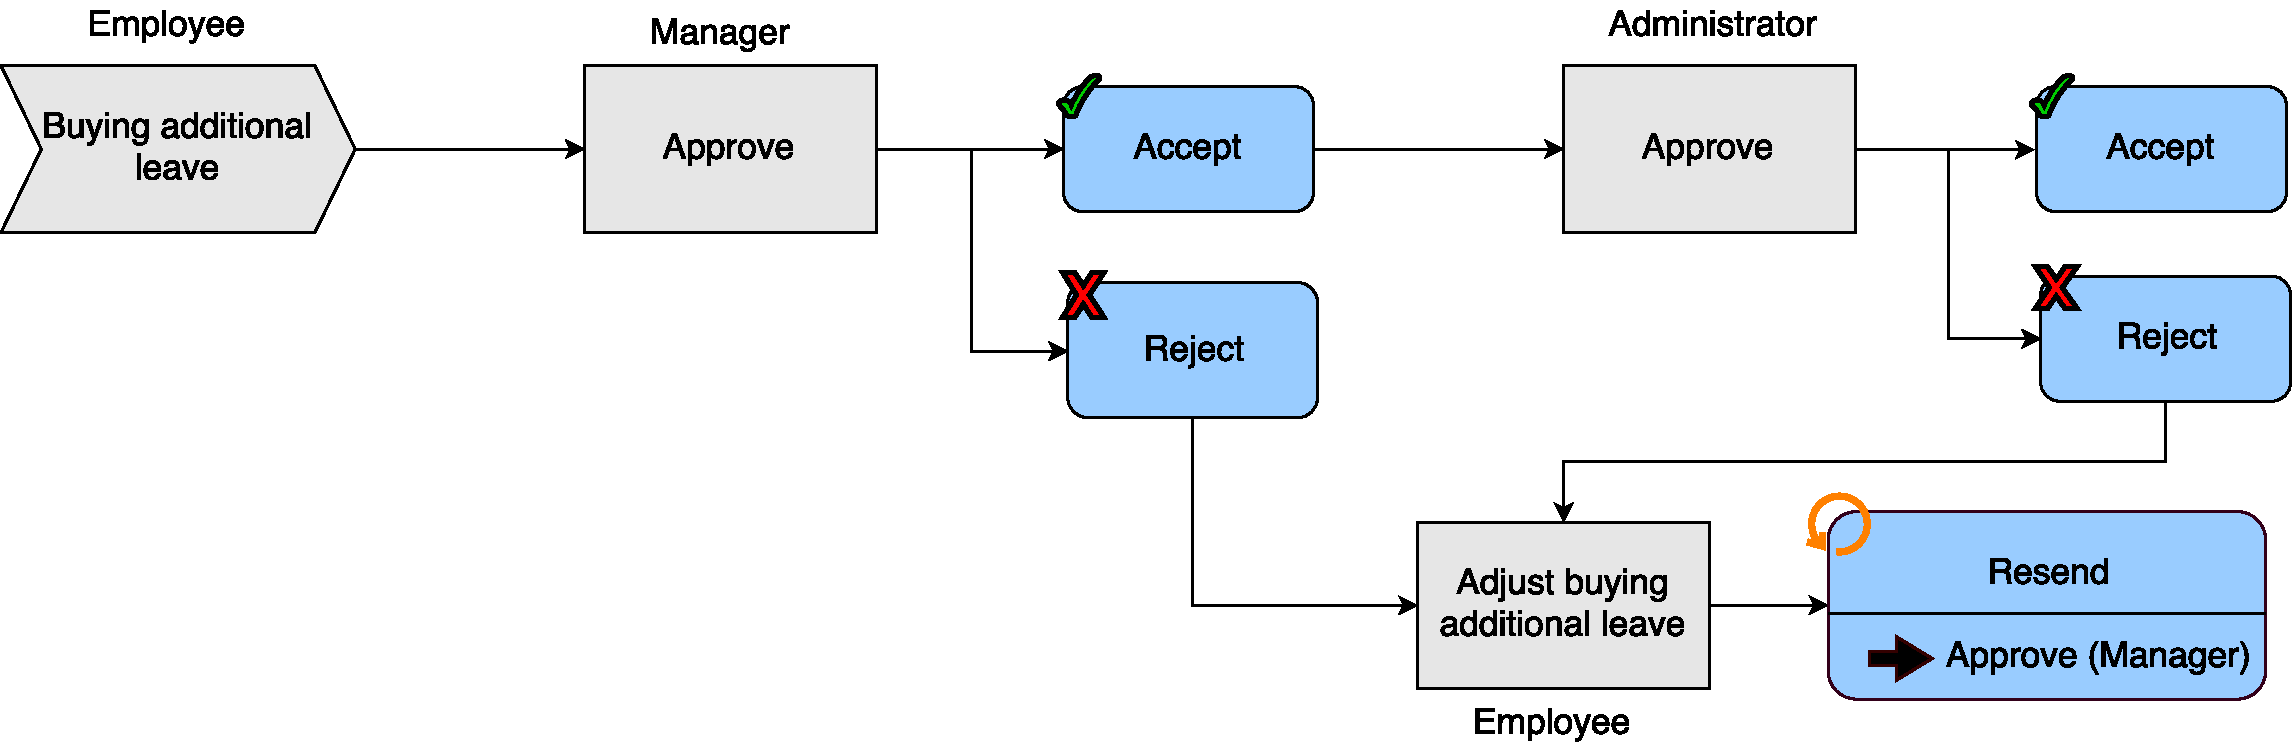
\includegraphics[width=\linewidth]{Example_Workflow.pdf}
\caption{Example workflow, representing the process of buying additional leave. Gray nodes are tasks, whereas blue nodes are actions. The dotted squares represent occurrences of the Approval pattern.}
\label{figure:example_workflow}
\end{figure}

In case one of the two approvers does not agree with the request, the employee needs to adjust his request. Note that the action \textit{Resend} refers to the task \textit{Approve}. This means that this action leads to the task \textit{Approve} (another way to show this functionality would be to simply add an arrow from \textit{Resend} to the leftmost \textit{Approve}). Finally, the workflow is completed when the rightmost \textit{Accept} action is executed.

Besides tasks and actions, there are workflow patterns. According to \cite{Patterns1996}, a pattern \textit{“is the abstraction from a concrete form which keeps recurring in specific nonarbitrary contexts”}. In other words, a pattern is an abstraction of a concrete set of tasks of actions and is independent of the workflow language used. An example is the or-split workflow pattern, which is visible in Figure \ref{figure:example_workflow}. Since the task \textit{Approve} has two actions and you may only choose one, you can see this structure as an OR-split.

The problem we try to solve, is to find certain patterns within such a workflow. However, we look beyond the purely syntactic scope of patterns and try to include the semantics or contextual meaning of a pattern (i.e. high-level workflow patterns). To give an example, we can say that the workflow in Figure \ref{figure:example_workflow} contains a pattern which we call the \textit{Approval pattern} ("accordeer patroon" in Dutch). In short, this pattern represents the decision whether some change in the system gets accepted or not. As you can see, such a decision occurs two times in the workflow example: the manager needs to approve the request and also the administrator needs to approve this (indicated as the dotted areas in Figure \ref{figure:example_workflow}). So when we try to find occurrences of the approval pattern, we would like to see these two parts of the workflow in the result of our query.

\subsection{Purpose Of This Study}
As a business company, you often can use workflows provided with your ERP-software package or create your own workflow. Provided workflow templates are in general workflows which represent very common business processes and most companies would like to use them. When you would like to have a workflow for a very specific process, you might have to assemble your own workflow structure. However, setting up such a workflow can become quite complex which can easily lead to errors in the model defined. Especially when you have to consider multiple different use cases.\\
To remove the burden of giving the user the option to define a workflow on such a low level by itself, we want to discover workflow patterns on a higher level. This way, we can abstract away from the low level representation of a workflow and use these high-level patterns to describe processes in an organization.\\
\\
In the eyes of an IT-company which develops and sells ERP-software, it is important to know which processes are most common in a company and what kind of steps are most important in workflows. Of course, having a good insight in the usage of workflows will be very helpful when you want to deliver a workflow management system. Getting a better understanding of the high-level workflow patterns \footnote{From now on, when we talk about workflow patterns, we mean high-level patterns as described here}, and their behavior, in workflow models is the goal of this research project.

\section{Preliminaries}
Let us state some basic definitions which we use throughout this thesis.
First of all, let us give a formal description of what a workflow (pattern) is.
\begin{defn}[Workflow]
A \textit{workflow W} is a set of tasks \textit{T} and corresponding actions $A$, set up to accomplish some business process.
\end{defn}

\begin{defn}[Workflow Pattern]
A \textit{workflow pattern p} is a subset of a workflow $W$, i.e. $p \subset W, a_p \in A, t_p \in T$, such that this pattern represents a specific objective $O$.
\end{defn}
Recall the ``Approving pattern" from the example workflow in Figure \ref{figure:example_workflow}, which consists of the task \textit{Approve} and actions \{\textit{Accept, Reject}\}. The objective $O$ is in this case the \textit{approval} of something.

\begin{defn}[Workflow pattern similarity]
Two workflow patterns $p$ and $p'$ are said to be similar if they represent the same objective $O$. Thus, $p=p'$ i.f.f. $p \rightarrow O \wedge p' \rightarrow O$.
\end{defn}

\begin{defn}[Petri net]
A petri net is a directed graph, consisting of places and transitions that are connected by arcs. From the literature study follows that Petri nets are a powerful and widely used representation for workflows. A petri representing a workflow is called a \textit{workflow net}, which is a petri net having just one start place and one end place (like a workflow should have). When a workflow consists of blocks which also have the property of starting and ending in one place are called \textit{block-structured}. 
\end{defn}


\section{Literature Study}
\label{section:literature}
This section discusses previous works, presenting theories and techniques around workflows, workflow patterns and the problem of mining such structures from workflow models.\\
\\
% Talk about process re-engineering in general and about workflows
Business process re-engineering is firstly proposed by \cite{AutomatingBusinessProcesses1990} as an approach to tackle the problem of improving the quality of business processes, while reducing their cost. One of the earlier works presenting workflow management systems are \cite{OfficeCommunicationsSystem79,OfficeInfoSystem1982}. The term \textit{information control net model} gets introduced by \cite{OfficeInfoSystem1982}, which can be seen as one of the earlier variants of workflow models. 

As I mentioned earlier, there are no real standards when it comes to the workflow paradigm \cite{VanderAalst1997Verification}. This causes that management systems use different modeling languages, but a more important problem is the ability of verifying and analyzing workflows is often not available in such tools \cite{VanderAalst1997Verification}. Because of this reason, \cite{VanderAalst1997Verification} shows that a class of \textit{Petri nets} can be used as a way to represent workflows, which they call \textit{WF-nets} (workflow nets). Also, the correctness of WF-nets can be analyzed using the Petri net theory. 

% Talk about workflow patterns

The most common way to verify whether a workflow language is a good representation is by checking which \textit{workflow patterns} are covered by this language. A workflow pattern is described by \cite{Patterns1996} as \textit{``the abstraction from a concrete from which keeps recurring in specific nonarbitrary contexts"}, which holds that a pattern represents a certain functionality in a workflow while being dependent of the modeling language. Many \cite{VanderAalst2003Patterns,Dijkstra2003ControlPatterns,Russell2004DataPatterns,Russell2005ResourcePatterns,Russell2006ExceptionPatterns} describe workflow patterns providing functional requirements for workflow model languages. As stated in \cite{VanderAalst2003Patterns,Dijkstra2003ControlPatterns,Russell2004DataPatterns,Russell2005ResourcePatterns,Russell2006ExceptionPatterns}, a workflow pattern is defined by (1) a set of conditions which must be satisfied to be applicable, (2) examples of business situations where this pattern should be applied, (3) a problem description stating why applying this pattern is not trivial and (4) implementation solutions. Unfortunately, there are no studies specific for the discovery of workflow patterns on a higher-level. The extension of the workflow pattern mining problem by including semantics is something we will be the first to do research on.

% Talk about workflow mining
Whereas the notion of process mining emerged within the last two decades \cite{VanderAalst2003Survey}, the concept of workflow mining is first introduced by \cite{WorkflowMining1998}, presenting an algorithm which has a set of unstructured executions of a business process as input, and outputs a minimal dependency graph representing the control flow of this business process. Furthermore, \cite{WorkflowMining1998} discusses ways to cope with cycles in the graph and noise in event logs (missing executions of tasks or wrongly inserted tasks in a log). Others heuristic approaches for noise and incomplete logs are presented in \cite{Maruster2002LogisticRegressionModel,Weijters2001DiscoveringWorkflowModels,Weijters2001Noise}. The heuristic approach \cite{Weijters2001DiscoveringWorkflowModels,Weijters2001Noise} is a combination of the following steps: (1) constructing a dependency/frequency table, (2) mining basic dependency relations out of this table and (3) creating a workflow based on the relations found. Besides using these steps, \cite{Maruster2002LogisticRegressionModel} presents a logistic regression model to learn when two events are direct dependencies of one another. 

\cite{VanDerAalst2002PetriNets} states that it is impossible to mine every possible WF-net. They name this challenge being the \textit{rediscovery problem}: \textit{``Find a mining algorithm able to rediscover a large class of sound WF-nets on the basis of complete workflow logs."}\cite{VanDerAalst2002PetriNets}. An algorithm which can successfully mine a large class of WF-nets is the $\alpha$-algorithm \cite{VanderAalst2003Survey,VanDerAalst2002PetriNets,VanderAalst2002TimedLogs}, which assumes that the given workflow log is complete (this means that every possible execution path of the business process at hand must be present in the log). Although this completeness requirement is easy to satisfy for a simple workflow, larger workflows will have more trouble. For instance, a workflow having 10 tasks which can be executed in parallel results in $10!=3628800$ possible execution sequences. As you can tell, there is a rather small chance that every possible sequence is covered in a corresponding workflow log. Besides, the $\alpha$-algorithm did have issues with loops and self-loops. Multiple extensions on the $alpha$-algorithm have been developed. like The $\alpha+$ variant \cite{A+-algorithm2004} which can deal with such short loops, and \cite{VanderAalst2002TimedLogs} which applies the algorithm on timed logs. Other approaches are the Heuristics miner, which can deal with noise \cite{HeuristicsMiner2006}, and the Inductive Miner \cite{InductiveMiner2013} that finds a sound and fitting process model in polynomial time.

% Talk about event logging formats

% Talk about word2vec
When we search for research done on determining semantic meanings of words, we see that this field has attracted a lot attention in the last few years. Especially the word2vec model \cite{Mikolov2013aWord2Vec,Mikolov2013bWord2Vec} is a popular technique. This technique results in a vector space representation of words which carries semantic meanings and is very useful in natural language processing tasks. Many variants on Word2Vec have been proposed, like Sent2Vec \cite{Sent2Vec}. Sent2Vec is particularly useful for our problem, since descriptions can exist of more than one word. The general idea behind Sent2Vec is computing the average vector of a sentence by looking the vectors up for each word through Word2Vec. However, applying Word2Vec as a way to determine the similarity between patterns in workflow models is something new.

% Talk about workflow(pattern) mining tools
A widely used tool for process mining is ProM \cite{ProM6} (at the time of writing the latest ProM version is 6.7). This open-source, extensible framework has over 600 different plug-ins, including process mining algorithms like the $\alpha$-algorithm, who add their own functionality to the complete software package. ProM gives the user lots of possibilities when it comes down to mining event logs and the user interface helps with getting a good understanding of the structure of process models. In the article \cite{WorkflowMiner2006} are rules shown which describe the sequence- fork- and join workflow patterns. Furthermore, they made a plug-in for ProM 5.2 called ``Workflow pattern miner". Another plug-in, called the "Inductive Miner" \cite{InductiveMiner2013}, is an implementation of the inductive mining algorithm on event logs. 

\section{Problem}
The challenge which we undertake in this thesis, is to reason about interesting patterns in a given collection of workflow event logs. As a case study, we use the data of the current product of our case company AFAS Software BV. AFAS is interested in the behavior of specific patterns and we hope to give them more insight about this as a result of this research. Note that we want to look further than the syntactic value of a pattern. We try to come up with a technique such that we can also mine patterns based on their semantics, which will give us a lot more information.\\
\\
During an iterative development, including meetings with domain experts of AFAS, we try to discover workflow patterns from which AFAS knows that they exist. However, the behavior of these workflow patterns are still unknown. To be able state that a pattern behaves in a certain way, we need to look at his occurrences in workflows modeled in Profit. Thus, by mining and analyzing occurrences of such patterns, we hope to find certain properties about these patterns. Which properties we will consider, differs from the pattern at hand and are expected to get more clear after discussions with domain experts at AFAS.\\
\\
As a result, this thesis will discuss which patterns we have studied and what conclusions about their behavior can be drawn, based on the occurrences found in the given workflow logs.\\
\\
If the analysis of the patterns known by AFAS is completely finished and we still have some time\footnote{See Section \ref{section:planning} for further information about my planning.} before the final deadline is reached, we will try to discover other patterns. By applying a frequent pattern discovery technique on the workflow models mined, we hope to find new patterns which were not already detected by the domain experts at AFAS.

\section{My Approach}
Since more than 10 years ago, workflow events are being logged in the software package Profit. These logs are essentially a table where every record represents an action on a task in a certain workflow instance. Although the logs contain more fields, the most relevant fields are shown in an example log in Table \ref{table:log}. The first field is the \textit{Workflow ID} and is a unique reference to a workflow model (task/action graph like in Figure \ref{figure:example_workflow}) where this event sequence is based on. Although I did not include more workflows in the example, there are many workflow models used, so this field is not trivial. By grouping on this field, you collect all event logs of that specific workflow log.

The \textit{Case ID} denotes the instance or event sequence of a given workflow. Another way to refer to an event sequence is by using a tuple $<\text{Workflow ID}, \text{Case ID}>$. The \textit{Task ID} is a key for the current task in the sequence. The \textit{Action ID} refers a unique action, given a task. Note that this value when you consider the complete workflow model. Every task within a workflow must have at least one action, and these action ID's all start at 1. The purpose of using these id fields will become more clear when I discuss the pre-processing steps planned on this data.

Then we also have two fields \textit{Task Description} and \textit{Action Description} which represent the actual meaning or reasoning behind a task or action in the workflow. These descriptions are words given by the creator of the workflow. Since we are interested in the context of such tasks or actions, these fields will become crucial for determining this context.
Finally, the last two fields \textit{Start Time} and \textit{End Time} contain the time stamps of this action. When you see a workflow as a finite state machine, the moment that the current task is entered is the start time of this state, whereas the moment that the action is triggered is the end time of this state. Using this information, we can derive the order of events in a sequence.

Using this information, we can derive that the log contains two event sequences, shown in Table \ref{table:example_sequences}. 

% Please add the following required packages to your document preamble:
% \usepackage{graphicx}
\begin{table}[H]
\centering
\caption{An example workflow event log.}
\label{table:log}
\resizebox{\textwidth}{!}{%
\begin{tabular}{|l|l|l|l|l|l|l|l|}
\hline
Workflow ID & Case ID & Task ID & Task Description               & Action ID & Action Description & Start Time     & End Time       \\
\hline
1           & 82      & 1       & Approve order (Manager)        & 1         & Accept             & 2-1-2017 09:10 & 2-1-2017 11:15 \\
1           & 82      & 2       & Approve order (Administrator)  & 1         & Accept             & 2-1-2017 11:15 & 2-1-2017 11:42 \\
1           & 83      & 1       & Approve order (Manager)        & 2         & Reject             & 2-3-2017 08:36 & 2-3-2017 08:49 \\
1           & 83      & 3       & Adjust buying additional leave & 1         & Resend             & 2-3-2017 08:49 & 2-3-2017 09:11 \\
1           & 83      & 1       & Approve order (Manager)        & 1         & Accept             & 2-3-2017 09:11 & 2-3-2017 09:17 \\
1           & 83      & 2       & Approve order (Administrator)  & 2         & Reject             & 2-3-2017 09:17 & 2-3-2017 09:33 \\
1           & 83      & 3       & Adjust buying additional leave & 1         & Resend             & 2-3-2017 09:33 & 2-3-2017 09:53 \\
1           & 83      & 1       & Approve order (Manager)        & 1         & Accept             & 2-3-2017 09:53 & 2-3-2017 10:04 \\
1           & 83      & 2       & Approve order (Administrator)  & 1         & Accept             & 2-3-2017 10:04 & 2-3-2017 10:11 \\
\hline
\end{tabular}%
}
\end{table}

% Please add the following required packages to your document preamble:
% \usepackage{graphicx}
\begin{table}[H]
\centering
\caption{Sequences of workflow with ID 1, based on the workflow log in Table \ref{table:log}.}
\label{table:example_sequences}
\resizebox{\textwidth}{!}{%
\begin{tabular}{|r|l|l|}
\begin{tabular}[c]{@{}l@{}}
Case ID $\rightarrow$\\ Step in workflow$\downarrow$\end{tabular} & 82                                     & 83                                     \\
\hline
1.        & Approve order (Manager) - Accept       & Approve order (Manager) - Reject       \\
2.        & Approve order (Administrator) - Accept & Adjust request - Resend                \\
3.        &                                        & Approve order (Manager) - Accept       \\
4.        &                                        & Approve order (Administrator) - Reject \\
5.        &                                        & Adjust request - Resend                \\
6.        &                                        & Approve order (Manager) - Accept       \\
7.        &                                        & Approve order (Administrator) - Accept
\end{tabular}%
}
\end{table}

Of course, we cannot start mining workflow patterns directly from workflow logs like described above. Some steps need to be made before mining techniques can be applied. Now that we have seen what kind of data we will be working with, let's discuss possible actions which translates this raw data into something we can use for mining high-level workflow patterns.

\subsection{Pre-Processing Phase}
First of all, the log needs to be ordered. This ordering is done in the following way

\begin{equation}
\text{Workflow ID} \downarrow \quad \text{Case ID} \downarrow \quad \text{Start Time} \downarrow \quad \text{End Time} \downarrow
\end{equation}

Applying this ordering results in a table where the records are chronologically ordered. This means that consecutive events within an instance of an workflow are placed together and their order goes from first to last event. 

Important to note is that we do not know the workflow model beforehand. Although the example log from Table \ref{table:log} is based on the model in Figure \ref{figure:example_workflow}, in general we do not have access to the corresponding model. Why you might ask? Well, Profit itself only contains templates and basic workflows, but many processes use a workflow which is further customized. Customers can change a standard workflow to their own wishes or make a complete new workflow model to fulfill their wishes. Since the configuration of workflows can be done by customer, these versions are not stored in one central unit, but every environment keeps track of the workflows it uses. Thus, we need to find a way to derive the workflow model from the event logs we obtained. More on this is explained later.

Another issue is that different versions of a workflow can be used throughout time. This means that different descriptions for tasks/actions can be used, or tasks/actions who previously existed in the model can be removed in later versions. Unfortunately, the event logs do not refer to a specific version of a workflow model. This causes a problem when mining for relations between tasks and actions. To give an example, recall the example workflow in Figure \ref{figure:example_workflow} and suppose that, at some point in time, the description of the first task ``Approve" gets changed to ``Check". The result of this change, is that all upcoming instances of the workflow log a task called ``Check", whereas we before logged ``Approve''. How do we determine that instances using ``Approve'' and instances using ``Check'' use a different workflow model? We can do this by iterating over all instances of a workflow, keeping track of a dictionary where we store the description of every task as a tuple $<\text{Task ID}, \text{Task Description}>$. By starting at the most recent instance, we collect the latest workflow model. When an instance uses a different description for a task, given the Task ID, then we conclude that its \textit{workflow version} is different. The same goes for changed actions in a model. This way, we can recognize which instances belong to the same workflow version. This recognition is very important, since we want to derive the correct model and this can only be done when we know which event sequences are based on this model. Using logs which used a different model will of course influence our mined model in a negative way, which is something we try to avoid.

\subsubsection{Word2Vec}
\label{section:word2vec}
For comparing two workflow patterns with each other, we will focus on a natural language processing technique, called Word2Vec model \cite{Mikolov2013aWord2Vec,Mikolov2013bWord2Vec}. The Word2Vec model translates a given corpus into a vector space. This means that each word in the corpus has a certain position, say vector, in this multi-dimensional space. The reasoning behind this is that different words who have the same context, are often shown to be very similar. Shown in Figure \ref{figure:word2vec_example}, `apple' and `pear' are likely to appear in the same region. However, we expect the word `car' to be positioned further away. The position of a so-called \textit{target word} is determined by its \textit{context words}. Context words are words that surround the target word. For instance, when you have the sentence ``Most of the time, apples are green" and you are interested in the positioning of the word `apples', then its context words are `the', `time', `are', `green'. Note that I used a context window of 2, meaning that only words maximum 2 words positioned from the target word are included in our context. However, you are free to define which words belong are contextual and experimenting with this definition is often needed in order to find the best results. 

To put Word2Vec in our perspective, terms which are used in descriptions of tasks and actions in the workflow models studied, will behave the same way. For instance, we expect that `approval' and `agreement' will lie pretty close to each other.

\begin{figure}[H]
\centering
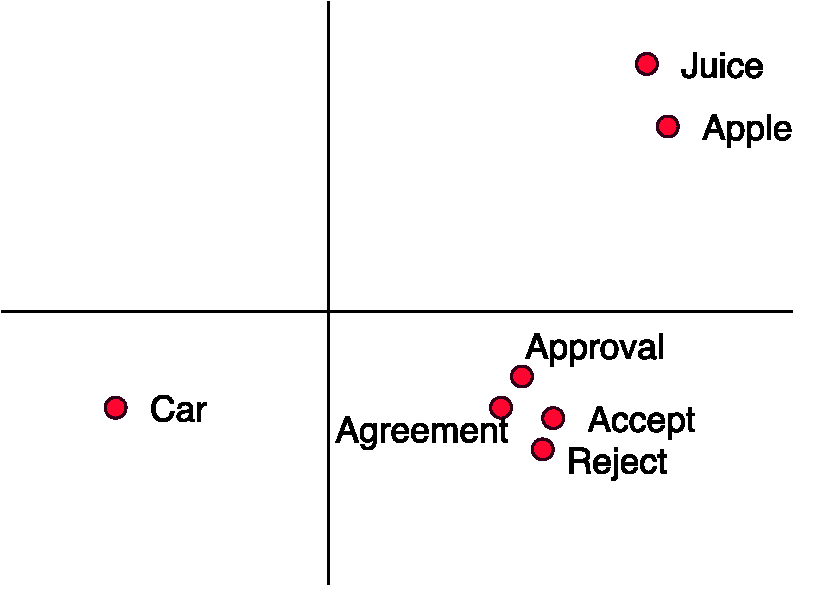
\includegraphics[width=0.6\linewidth]{word2vec_example.pdf}
\caption{An example vector space.}
\label{figure:word2vec_example}
\end{figure}

Since descriptions of tasks and actions can contain multiple words, we will use a variation of Word2Vec, called \textit{Sent2Vec} \cite{Sent2Vec}. Sent2Vec is a way to train distributed representations of sentences. In short, Sent2Vec uses an aggregate function to determine the vector of a sequence of words. For example, you can define the final vector as the average vector when applying Word2Vec on each word in the sentence. So when looking at our example sentence $s=$``Most of the time, apples are green", you can say that 
\begin{equation}
v(s)= \frac{1}{7} * [v(\text{most})+v(\text{of})+v(\text{the})+v(\text{time})+v(\text{apples})+v(\text{are})+v(\text{green})].
\end{equation}

Using this technique, we can train a vector space on the words used in the workflow logs and check whether the words used in the workflow patterns are similar or have very different positions. Question which we did not answer yet are:

\begin{enumerate}
\item On what level do we apply Sent2Vec on a workflow model?
\item When do we conclude that two sentences are the same, given their vectors?
\end{enumerate}

As a first try, we will apply Sent2Vec on event level. This means that we consider the task- and action description of one event as a sentence and translate this sentence to a vector. As an example, recall Table \ref{table:example_sequences}, we could say that a sentence consists of the task- and action description of an event, like ``Adjust request - Resend". Then, we train the model such that events using the similar terms will lay close together in the resulting vector space if they have similar words in the task- and action description. This way, we expect that similar events are grouped together. However, it is very likely that the information needed to train a proper vector space differs per workflow pattern we study. For instance, it could be that we also need to include event occurring before or after the `target' event. It is impossible to explain this hard black-on-white at this stage and experimenting with different setups will solve this question.

Since the similarity of terms will be determined based on their positions in the vector space, the exact definition of similarity between such patterns will be given in a later stage of this study.

Before answering the second question, we need further explanation on how we define a workflow model and how we compare such models with each other. 

\subsubsection{The XES Event Log Format}
Since 2011, the standard event log format is XES \cite{XES2010Buijs}, which stands for \textit{eXtensible Event Stream}. This format is XML-based and many tools, like ProM 6+ \cite{XES2011Verbeek}, and algorithms, like the Inductive Miner \cite{InductiveMiner2013}, are based on XES files as their input. The logs like Table \ref{table:example_sequences} can easily be converted to this format. ProM contains an import Framework which can convert CSV files into XES files \cite{XES2011Verbeek}. 

\subsection{Workflow Mining Phase}
After completing the pre-processing steps, it is time to find workflow models and mine patterns from these models. As you can read in Section \ref{section:literature}, there are many existing techniques for mining the process model based on a given workflow log. The most complete technique is the Inductive Miner \cite{InductiveMiner2013}, since it always finds a sound, fitting model in a finite time. Therefore, we will use this technique in the phase of obtaining workflow models. Fortunately for us, this technique is implemented as a plug-in of the ProM framework \cite{InductiveVisualMiner2014}, which will be very useful to explore. Let me briefly explain how this algorithm works. 

The inductive miner uses a workflow log as input. Then, it determines the most likely split between the different events in the log in a divide-and-conquer approach. As an example, look at Table \ref{table:inducExampleLog}. The first split is applies is between $a$ and the rest, since it observes that every case starts with event $a$. The same can be said for $g$, which is the final event for every case. Then, the inner part of every case either ends with $e$ or $f$, which implies that there is an exclusive choice between $e$ and $g$. Lastly, the part that remains is a parallel relation between $b,c$ and $d$, since these events always occur, but their order is not fixed.

Based on these splits, the algorithm sets up a so-called \textit{process tree} \cite{Buijs2012ProcessTrees}, which is a compact abstract representation of a workflow net (recall that a workflow net is a petri net having one start place and one end place). A process tree is a rooted tree where nodes represent an operator and leaves represent events. Leaves with the same parent share a certain relation, which is defined in their parent. See Figure \ref{figure:processTree} for a concrete example.

\begin{table}[H]
\centering
\begin{tabular}{l|l}
Case & Events          \\
\hline
1.   & $<a,b,c,d,e,g>$ \\
2.   & $<a,b,c,d,f,g>$ \\
3.   & $<a,c,d,b,f,g>$ \\
4.   & $<a,b,d,c,e,g>$ \\
5.   & $<a,d,c,b,f,g>$
\end{tabular}
\quad
\begin{tabular}{l|l}
Split & string representation  \\
\hline
1.     & $\rightarrow(a)$  \\
2.     & $\rightarrow(a, g)$    \\
3.     & $\rightarrow(a, \times(e,f), g)$    \\
4.     & $\rightarrow(a, \wedge(b,c,d),\times(e,f), g)$   \\    
\end{tabular}
\caption{Example log, shown in the left table. On the right, you see the string representation of the resulting process tree, after a certain split.}
\label{table:inducExampleLog}
\end{table}

The inductive mining algorithm uses a set of operators. Some standard operators are:
\begin{itemize}
\item $\rightarrow$ means a sequential relation between its events.
\item $\times$ represents an exclusive choice between its events.
\item $\wedge$ means a parallel execution between its events.
\end{itemize}

These operators are used in the string representation of the process tree. On the right subtable of Table \ref{table:inducExampleLog}, these representations are shown after each split discussed. Eventually, we end with the process tree $\rightarrow(a, \wedge (b,c,d),\times(e,f),g)$. Note that Figure \ref{figure:processTree} describes the same relations. You should read this tree like: (1) first event $a$ is executed, (2) then $b,c$ and $d$ are executed in parallel, (3) then $e$ or $f$ are executed but not both, and finally (4) $g$ is executed, ending a case. 

\begin{figure}[H]
\centering
\begin{tikzpicture}[scale=2]
\node {$\rightarrow$} [grow=down]
child {node {a}}
child {node {$\wedge$}
child {node at (0.8, 0) {b}}
child {node at (0,0) {c}}
child {node at (-0.8, 0) {d}}}
child {node at (0.3, 0){$\times$}
child {node at (0.4,0) {e}}
child {node at (-0.2, 0) {f}}}
child{node{g}
};
\end{tikzpicture}
\caption{Resulting process tree from splitting the log shown in Table \ref{table:inducExampleLog}.}
\label{figure:processTree}
\end{figure}


You might wonder why process trees are so important, whereas so much research \cite{VanderAalst2003Survey} is done on other modeling languages (petri nets, BPMN, YAWL etc.). However, these standard business process model languages allow the occurrence of anomalies such as deadlocks, live-locks and improper termination \cite{Buijs2012ProcessTrees}. Since such properties can only be checked afterwards, it is quite hard to ensure the soundness property when such a model gets constructed. Process trees do not have this drawback, because of their block-structure \cite{2009DifferenceBetweenGraphAndBlockStructuredLanguages}. This means that every possible process tree is a sound model, which is something we cannot say about petri nets or other types of models.

\subsection{Finding Patterns in Process Trees}
\label{section:occurrences}
Eventually we obtain process trees from the set of workflow logs used as input. Then it is time to mine the occurrences of a given workflow pattern $p$ in a mined process tree $T$. Assuming that this pattern $p$ is given as a process tree, we can search whether $p$ is a subtree in a process tree $T$ in our dataset, i.e. $p \in T$. Here it is needed to know which constraints have to be met in order to conclude that $p$ is contained in $T$. In general, the following two types of subtrees are mostly used (based on definitions given in \cite{FREQT2010Survey}):
\begin{itemize}
\item \textit{Induced subtrees}: An induced subtree $T'$ from tree $T$ is defined by the following constraints:
\begin{enumerate}
\item $V' \underline{\subset} V$, where $V'$ and $V$ are the sets of vertices for $T'$ and $T$ respectively.
\item $E' \underline{\subset} E$, where $E'$ and $E$ are the sets of edges for $T'$ and $T$ respectively.
\item Each vertex $v' \in V'$ is mapped one-to-one to a vertex $v \in V$. The same counts for all edges in $E'$.
\item Possible ordering of siblings in $T'$ is preserved in $T$.
\end{enumerate}
\item \textit{Embedded subtrees}: An embedded subtree $T'$ 
\end{itemize}

\subsection{Developing a Tool}
Since we want to apply these techniques on a large scale, we need to develop a program that is able to apply the techniques mentioned - given a collection of workflow logs and workflow pattern - and deliver a set of workflow models containing this pattern. Let me go through the components which together form the whole process of retrieving relevant models from workflow logs:

\begin{enumerate}
\item The first step in this case study is applying pre-processing steps on the available data. This means that we want the available workflow event data to be structured in such a way, that we can apply existing workflow mining algorithms on it to discover causal relations between tasks in a workflow. This phase does not merely consist of filtering noise or sorting/grouping the data in a certain way, but also the challenge of capturing the semantics of events will be tackled. As explained in Section \ref{section:word2vec}, we will use Word2Vec \cite{Mikolov2013aWord2Vec,Mikolov2013bWord2Vec} as solution for this problem.

For the application of Word2Vec, we have multiple options. Java also supports the use of word2vec models. An option is to use DeepLearningJ \footnote{https://deeplearning4j.org/word2vec}, which is a library in Java and an implementation of word2vec. Alternatives are Gensim\footnote{https://radimrehurek.com/gensim/} (a python library) and Google's word2vec tool\footnote{https://code.google.com/archive/p/word2vec/}. 
\item After the vector space model is trained on the descriptions of the available workflow logging data, we can start with the actual mining phase. During this phase, we will try to find occurrences of a given workflow pattern. However, this can only be done when we have structured a workflow event log into a workflow model. When we have obtained the corresponding workflow model, we can properly search for the pattern we are interested in. Obtaining a workflow model in terms of a process tree will be done by applying the Inductive Miner algorithm \cite{InductiveMiner2013}. This algorithm is implemented in plug-ins since ProM 6.4 \cite{InductiveVisualMiner2014}, so we plan to use their corresponding source code. Fortunately for us, plug-ins in ProM are also accessible through a command-line approach\footnote{\href{https://dirksmetric.wordpress.com/2015/03/11/tutorial-automating-process-mining-with-proms-command-line-interface/}{(link to) Tutorial: Automating Process Mining with ProM’s Command Line Interface}}. This way, we hope to call the plug-ins we want to use (like the ``CSV to XES" plug-in \cite{XES2011Verbeek} and ``Inductive Miner" plug-in \cite{InductiveMiner2013}) without having to write our own implementation.
\item When we have collected the corresponding process trees, then the last step is to go through each of them and check whether the workflow pattern at hand occurs in this tree. Recall that the conditions for this check are discussed in Section \ref{section:occurrences}. Lastly, the models which contain the pattern are returned. 
\end{enumerate}

\section{Project Planning}
\label{section:planning}
This section describes the further planning of this research study. The official starting date of the project is February 12, 2018. The final date of the thesis is July 6, 2018. This period consists of 21 weeks in total, from which I have included 19 weeks in my planning. In short, the planning consists of three phases, as shown in Figure \ref{figure:planningOverview}. Since I find it quite naive to think that everything will go smoothly, the remaining 2 weeks are not included. It can be that these 2 weeks are needed at some point due to possible delay or personal reasons like illness.

In the remaining of this section, the three phases of the proposed planning are further discussed.

\subsection{Phase 1: Getting Started}
The first phase consists of three blocks (note 1a, 1b and 1c). Let me explain the different objectives:
\begin{itemize}
\item The thesis needs to include a description of the theories and techniques used. I will write this description at the beginning of the thesis, since I find it important to know that I understand the algorithms I use and the initial phase is the best moment to study this.
\item Furthermore, I start with the development of a tool which applies the algorithms explained on a given dataset (collection of XES files) $D$ and a workflow pattern $p$. Since we are interested in occurrences of $p$, the goal of this tool is to return all workflow models $m \in D$ which contain $p$.
\item Besides the previous points, I will try to set up a query which will be used to collect all relevant workflow log data needed. Since I already have access to the AFAS workflow logs, I will use that collection until I get data about other (client) environments. Eventually, I hope to have access to workflow logs from approximately 100 (large) client environments. This way, we expect to capture a wide range of workflow behavior, since the workflow logs are based on different, independent sources.

Furthermore, we need a workflow pattern to study. Although this step is also included in Phase 2, I believe that knowing a workflow pattern in Phase 1 will also help the development of the tool. Because of this reason, I also included the discussion of the first pattern in Phase 1.
\end{itemize}

The three blocks will be executed in parallel. I prefer working interchangeably between them, instead of focusing on only one block at a time. Furthermore, the early development of the tool will also lead to earlier results and makes it possible to retrieve feedback of domain experts in an early stage of the process.

\subsection{Phase 2: Iterative planning}
The second phase is the period where I work closely with domain experts at AFAS and we study one workflow pattern at a time. As you can see, Phase 2 in Figure \ref{figure:planningOverview} contains a repeat sign. This means that steps 2a, 2b, 2c and 2d get repeated in the process. At first, we need to define the workflow pattern we are interested in and set up hypotheses linked to its expected behavior (step 2a). Then, the tool is run and collects workflow models which contain occurrences of this pattern (step 2b). (step 2c) These models are its output and need evaluation by domain experts who can conclude whether or not the occurrences of the pattern at hand are indeed included in these models. (step 2d) If that is the case, then we can use these models for answering the corresponding hypotheses . If it is not the case, then we can have multiple causes:
\begin{itemize}
\item The pattern is not defined correctly. In this case, we need to change its definition and redo the process from step 2b.
\item The tool does not recognize occurrences of this pattern correctly. Then we need to tweak parameters of the corresponding algorithms and try again.
\item The pattern uses information which we do not have. In order to recognize its occurrences, it is needed that we include extra information in the process, which we do not have. In this case, we might consider to include such information fields into our query, recollect workflow log data and try again. Otherwise, it might be best to drop this pattern since it is to complicated to recognize.
\end{itemize}

The total amount of time which can be spent on this phase is set to 12 weeks. In the case that we run out of specific workflow patterns within this period, we can try to mine remaining patterns by the application of frequent subtree mining, as is stated in step 2*. With this optional step, we hope to discover patterns which are completely unknown at AFAS and gives us further insight in the usage of workflows by the customer.

\subsection{Phase 3: Finalizing thesis}
In the final stage, the process of studying workflow patterns is stopped and the focus lies on further completion of the thesis report itself and on the thesis defense. This period of 3 weeks should give me enough time to finish the thesis properly.

\begin{figure}[H]
\centering
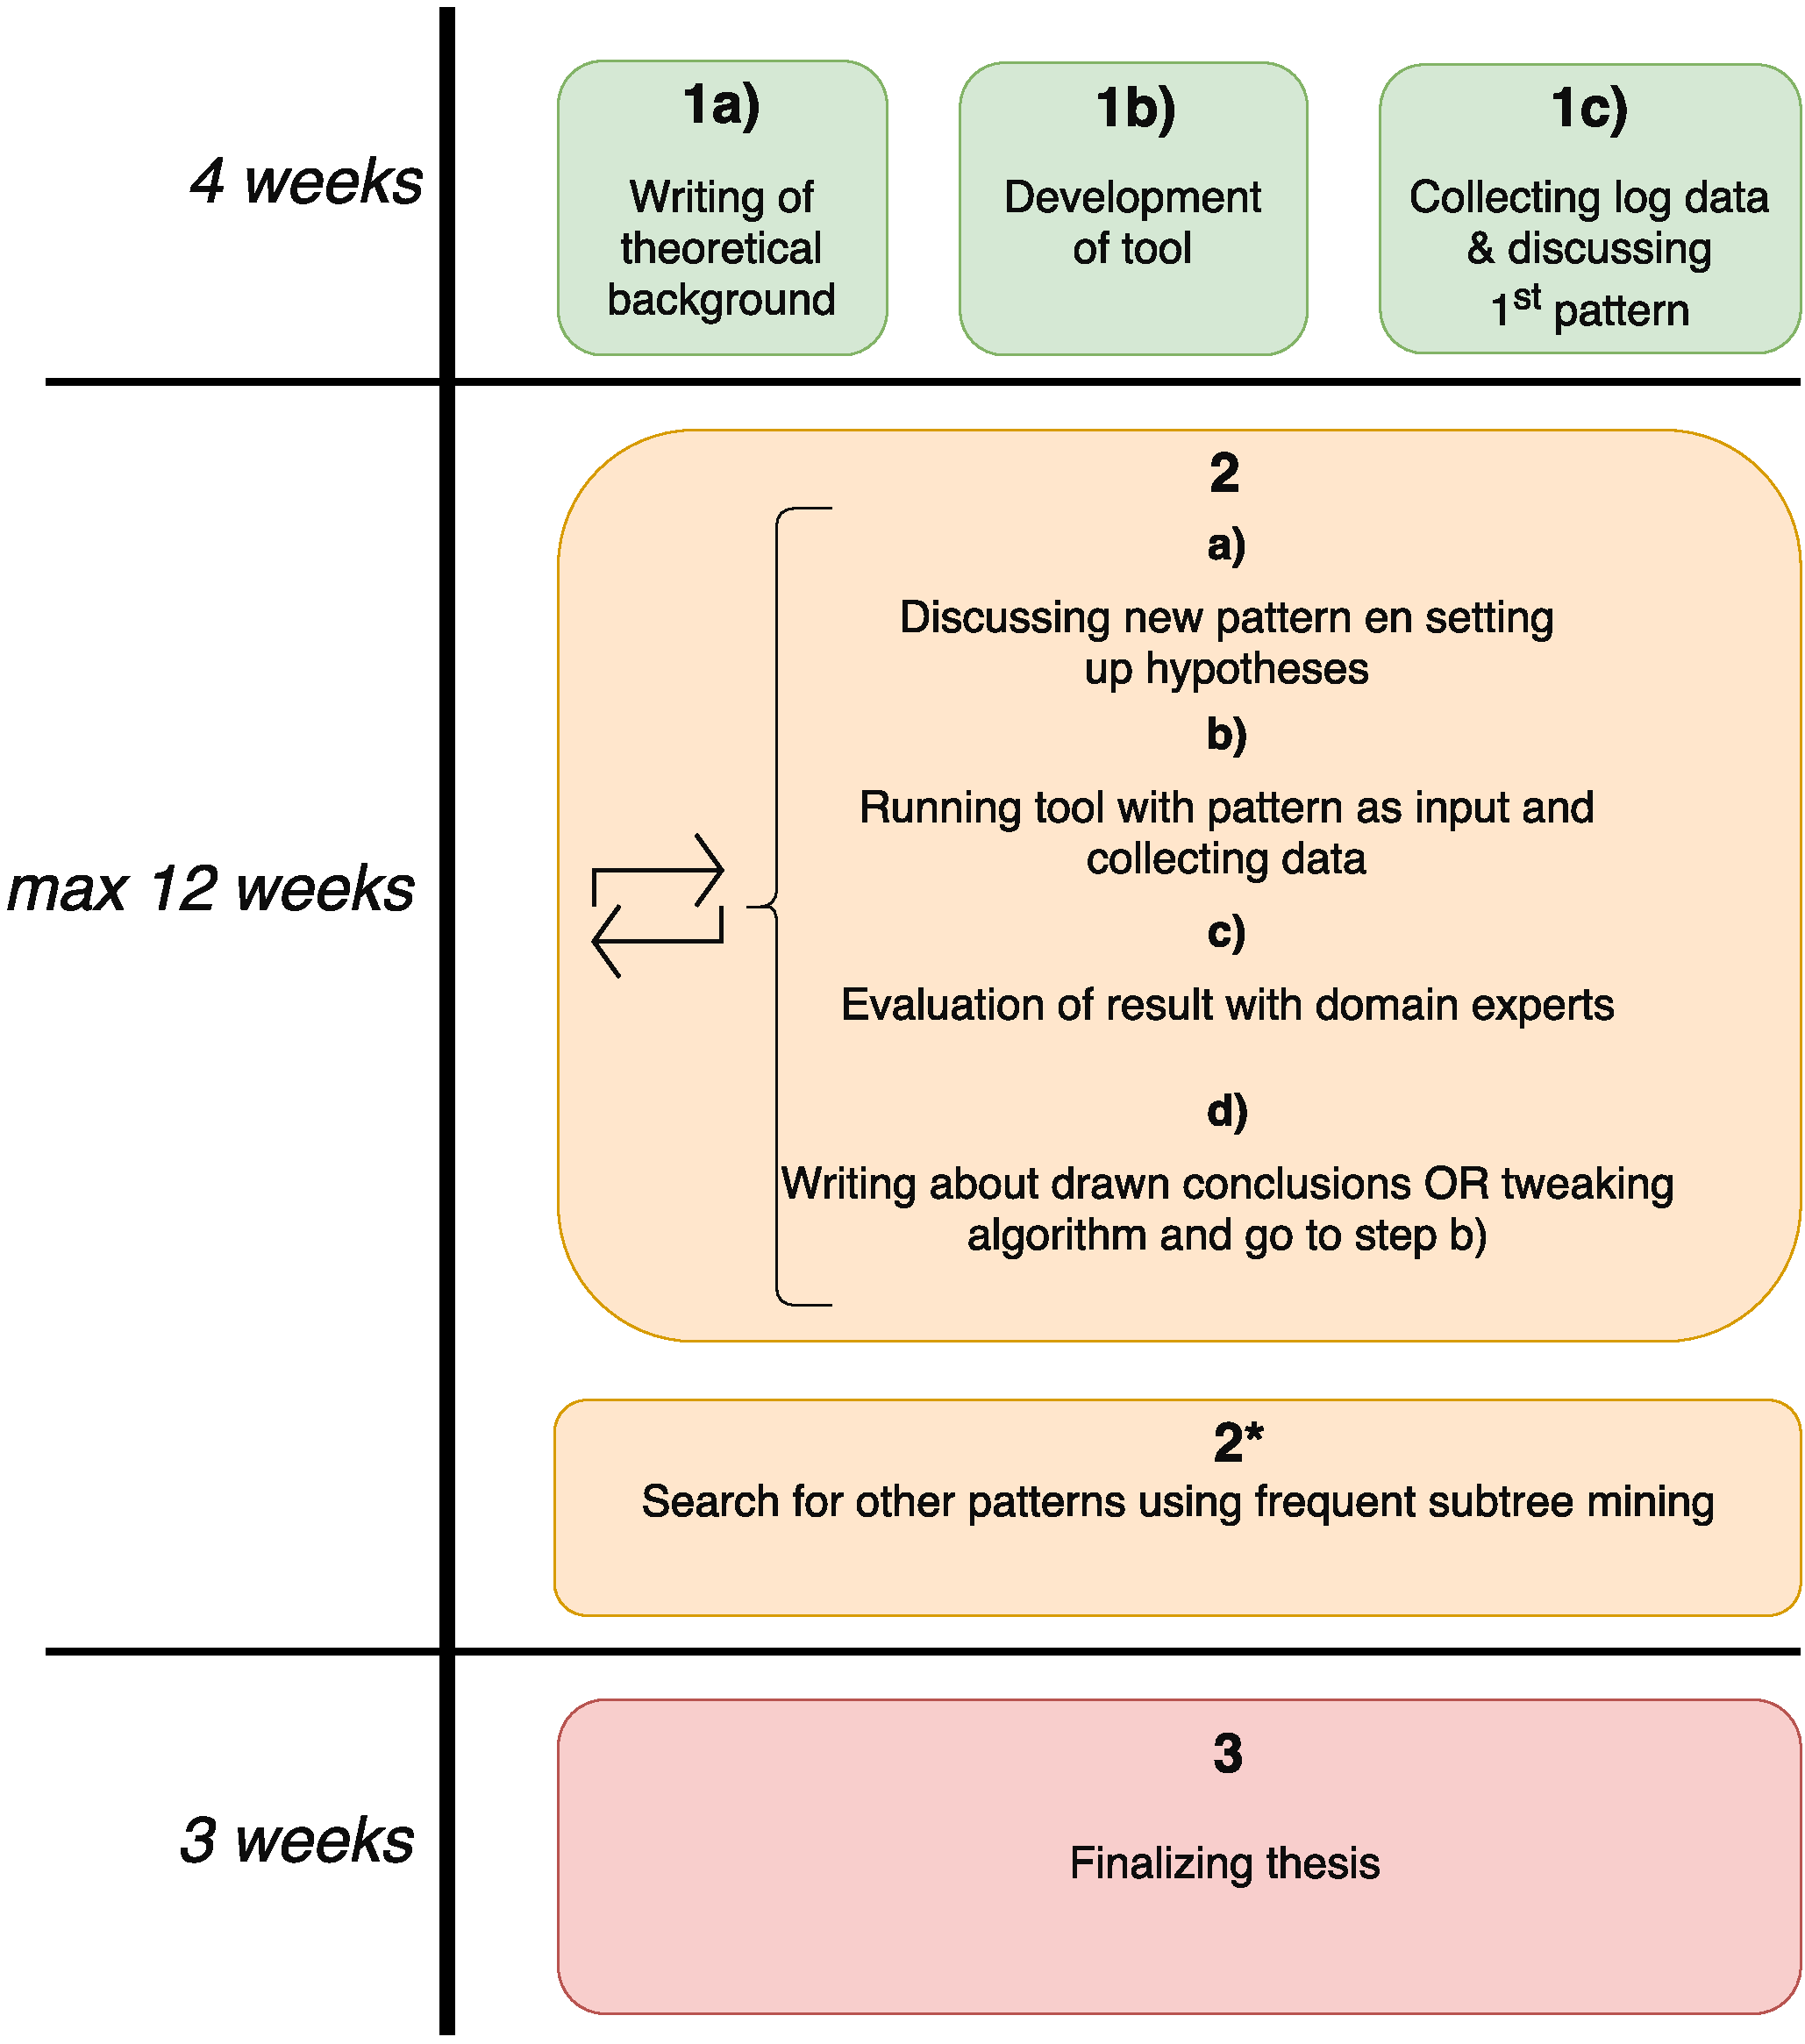
\includegraphics[width=.7\linewidth]{Planning.pdf}
\caption{High-level overview of the planned development of this thesis.}
\label{figure:planningOverview}
\end{figure}

\bibliographystyle{unsrt}
\bibliography{sources}

\end{document}